\chapter{Kiến thức và công nghệ nền tảng}
\label{chap:coso}

Chương này trình bày các kiến thức nền tảng mà Farmery vận dụng: bối cảnh chính sách và tiêu chuẩn chất lượng nông sản tại Việt Nam, các lý thuyết về mô hình thương mại điện tử, chuỗi cung ứng, truy xuất nguồn gốc, uy tín và công nghệ nền tảng, cùng các bài toán trí tuệ nhân tạo được tích hợp vào hệ thống. Các nền tảng và nghiên cứu cụ thể có liên quan được khảo sát riêng tại Chương~\ref{chap:lienquan}.

\section{Bối cảnh chính sách và tiêu chuẩn chất lượng nông sản}
\label{sec:boicanhchinhsach}

Chương trình OCOP (Mỗi xã một sản phẩm) là chương trình quốc gia hỗ trợ chuẩn hóa và nâng cao giá trị sản phẩm nông thôn/nông sản đặc trưng vùng miền. Hình~\ref{fig:ocop} tổng hợp số liệu tăng trưởng từ 2024 đến 2025 \parencite{danviet_2024_ocop, vietnamnet_2025_ocop}. Giai đoạn 2026--2030, chương trình được định hướng chuyển trọng tâm ``từ số lượng sang chất lượng'', trong đó đẩy mạnh số hóa sản xuất, truy xuất nguồn gốc và tiêu thụ qua thương mại điện tử được xác định là một trong các trụ cột \parencite{vietnamnet_2025_ocop} --- đây là tín hiệu chính sách thuận lợi cho định hướng của Farmery, đồng thời cũng là nguồn cung sản phẩm có thương hiệu và câu chuyện xuất xứ, phù hợp để đưa lên một sàn TMĐT có tính năng truy xuất nguồn gốc.

\begin{figure}[H]
\centering
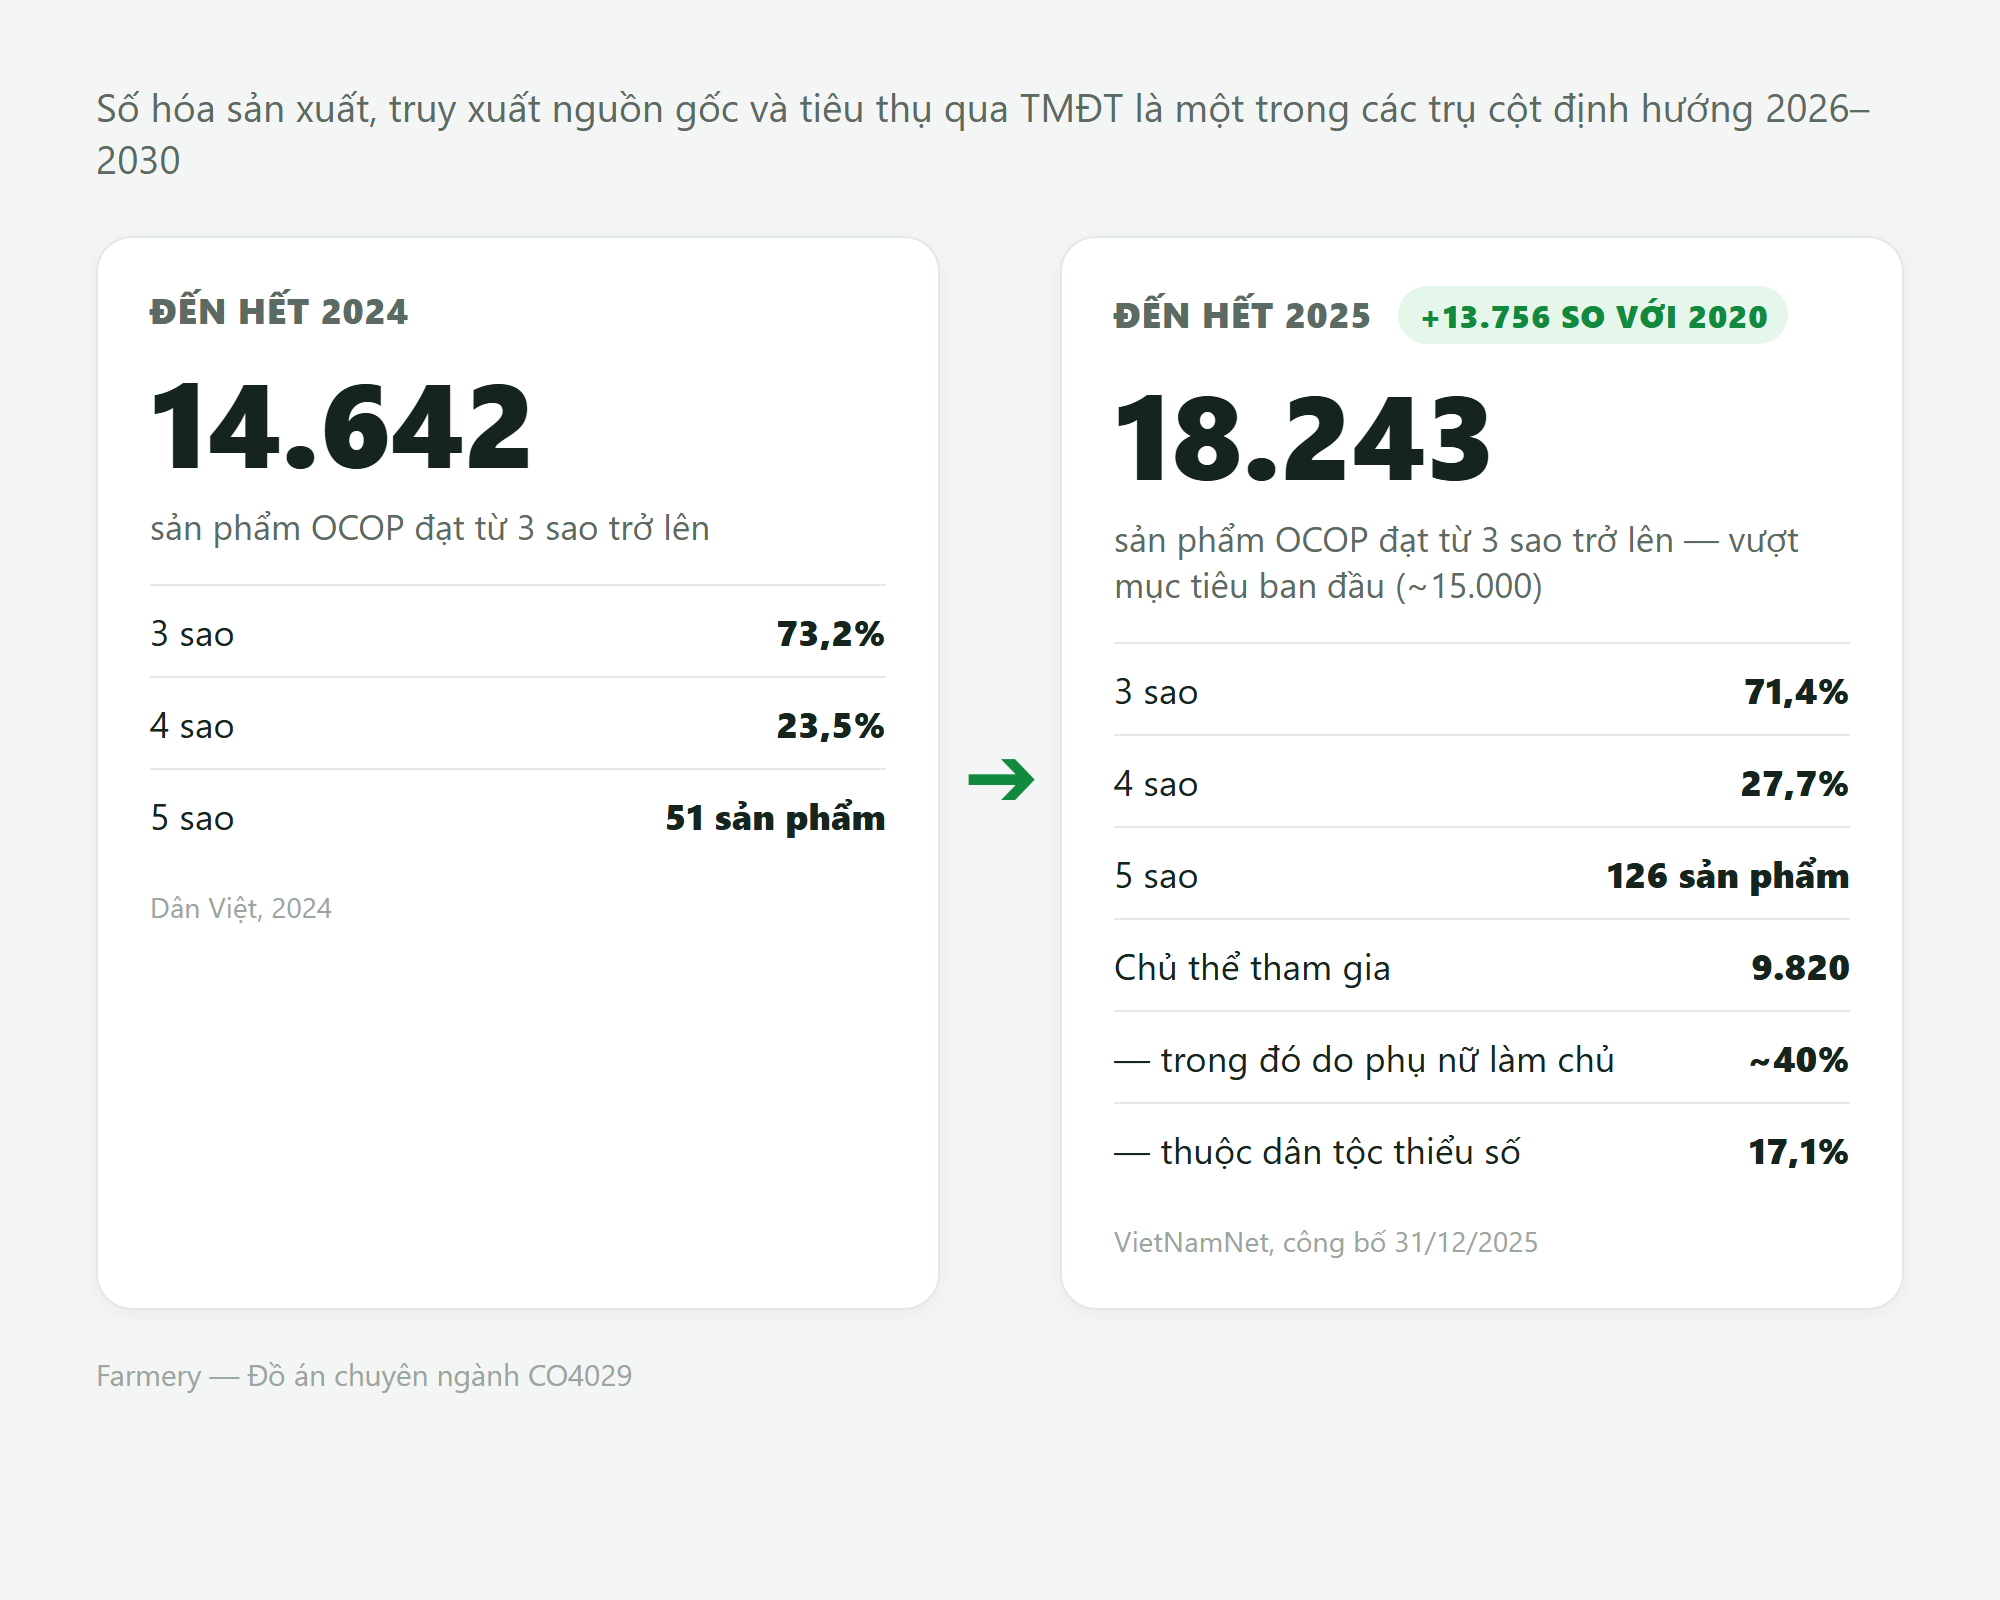
\includegraphics[width=\textwidth]{image/comparison/ocop-2024-2025.png}
\caption{Tăng trưởng của chương trình OCOP giai đoạn 2024--2025}
\label{fig:ocop}
\end{figure}

Về chính sách, các văn bản dưới đây lần lượt xác định nông nghiệp là lĩnh vực ưu tiên chuyển đổi số ở Việt Nam:
\begin{itemize}
    \item \textbf{Quyết định số 749/QĐ-TTg (03/6/2020)} của Thủ tướng Chính phủ phê duyệt ``Chương trình Chuyển đổi số quốc gia đến năm 2025, định hướng đến năm 2030'', xác định nông nghiệp là một trong 8 lĩnh vực ưu tiên (cùng Y tế, Giáo dục, Tài chính-Ngân hàng, Giao thông vận tải-logistics, Năng lượng, Tài nguyên-Môi trường, Sản xuất công nghiệp), với mục tiêu: phát triển nông nghiệp thông minh/chính xác; xây dựng dữ liệu lớn về đất đai, cây trồng, vật nuôi, thủy sản; tự động hóa sản xuất và quản lý chuỗi cung ứng; thúc đẩy TMĐT nông sản; và định hướng ``mỗi nông dân là một thương nhân'' \parencite{qd749_2020}.
    \item \textbf{Nghị quyết số 57-NQ/TW} của Bộ Chính trị về đột phá phát triển khoa học, công nghệ, đổi mới sáng tạo và chuyển đổi số quốc gia, tiếp tục là động lực cho chuyển đổi số ngành nông nghiệp trong giai đoạn mới \parencite{nq57_tw}.
    \item \textbf{Quyết định số 5943/QĐ-BNNMT (31/12/2025)} của Bộ Nông nghiệp và Môi trường (Bộ NN\&MT --- cơ quan hợp nhất từ Bộ NN\&PTNT và Bộ Tài nguyên-Môi trường từ 01/3/2025 \parencite{botnmt_2025}) phê duyệt kế hoạch chuyển đổi số ngành, với mục tiêu: 100\% thủ tục hành chính đủ điều kiện lên trực tuyến toàn trình (tối thiểu 85\% hồ sơ xử lý trực tuyến), dữ liệu chỉ khai báo một lần; cơ sở dữ liệu dùng chung nông nghiệp--môi trường; và ứng dụng dữ liệu lớn/AI trong giám sát, dự báo sản xuất \parencite{qd5943_2025}. Đây là văn bản chính sách cập nhật nhất, cụ thể hóa thêm định hướng tại Quyết định 749/QĐ-TTg và là căn cứ để Farmery khẳng định tính phù hợp với định hướng vĩ mô của Nhà nước.
\end{itemize}

Về tiêu chuẩn chất lượng, VietGAP và GlobalGAP là hai chuẩn thực hành nông nghiệp tốt mà Farmery dùng làm căn cứ kiểm duyệt chứng nhận:
\begin{itemize}
    \item \textbf{VietGAP} (Vietnamese Good Agricultural Practices) --- tiêu chuẩn trong nước, khoảng 70 tiêu chí, phù hợp chuỗi cung ứng nội địa (siêu thị, bếp ăn tập thể, chợ đầu mối).
    \item \textbf{GlobalGAP} --- tiêu chuẩn quốc tế nghiêm ngặt hơn, 252 tiêu chuẩn (36 tiêu chí bắt buộc 100\%, 127 tiêu chí tối thiểu 95\%, 89 tiêu chí khuyến nghị), là điều kiện tiếp cận thị trường khó tính (EU, Nhật Bản, Hàn Quốc, Úc, Mỹ); sản phẩm đạt chuẩn được gán mã định danh GGN 13 chữ số trong cơ sở dữ liệu toàn cầu, truy xuất minh bạch hơn VietGAP.
\end{itemize}
Một cơ sở đạt GlobalGAP đã vượt chuẩn VietGAP nên không cần chứng nhận VietGAP riêng; VietGAP thường là bước đệm năng lực trước khi nông dân/HTX tiến tới GlobalGAP nếu có định hướng xuất khẩu \parencite{vietgap_globalgap}. Đây là căn cứ để Farmery thiết kế quy trình kiểm duyệt chứng nhận theo 2 cấp độ (nội địa/VietGAP và xuất khẩu/GlobalGAP) tương ứng với 2 nhóm khách mua lẻ và mua sỉ B2B.

\section{Cơ sở lý thuyết nền tảng}
\label{sec:lythuyet}

\subsection{Mô hình thương mại điện tử B2C, B2B, B2B2C và marketplace nhiều người bán}

Trong thương mại điện tử, các mô hình được phân loại chủ yếu theo bản chất của các bên tham gia giao dịch. B2B (Business to Business) là mô hình kinh doanh giữa các doanh nghiệp với nhau, đặc trưng bởi các đơn hàng số lượng lớn và tính chuyên nghiệp cao thông qua hợp đồng. Trái lại, B2C (Business to Consumer) là mô hình kinh doanh giữa doanh nghiệp và người tiêu dùng cá nhân. B2B2C (Business to Business to Consumer) là một mô hình lai (hybrid), kết hợp giữa B2B và B2C, trong đó một doanh nghiệp cung cấp sản phẩm hoặc dịch vụ cho một doanh nghiệp khác, và doanh nghiệp thứ hai này sẽ bán trực tiếp cho người tiêu dùng --- đây là mô hình phổ biến trong các nền tảng thương mại điện tử như các sàn giao dịch trực tuyến. Ngoài ra, Multi-vendor marketplace (sàn nhiều nhà cung cấp) là mô hình thương mại điện tử cho phép nhiều người bán (vendor) đăng ký, đăng sản phẩm/dịch vụ, quản lý đơn hàng và nhận thanh toán trên cùng một nền tảng; người sở hữu sàn (marketplace operator) đóng vai trò quản trị, định ra quy tắc, thu phí và đảm bảo trải nghiệm mua bán liền mạch.

Farmery lựa chọn mô hình B2B2C dạng marketplace nhiều người bán nhằm đáp ứng nhu cầu mua nông sản của 2 tệp khách hàng khác nhau: người tiêu dùng cá nhân mua lẻ và doanh nghiệp mua sỉ theo hợp đồng từ nguồn cung là nông dân/hợp tác xã, còn nền tảng sẽ đóng vai trò trung gian cung cấp công nghệ, là nền tảng thanh toán và là nơi đáng tin cậy để đảm bảo các giao dịch diễn ra đúng quy trình, mang lại lợi ích cho các bên.

\subsection{Lý thuyết chuỗi cung ứng nông sản ngắn (SFSC) và disintermediation}

Chuỗi cung ứng thực phẩm ngắn (SFSC), theo định nghĩa của EU, là một chuỗi cung ứng liên quan đến một số lượng hạn chế các nhà điều hành kinh tế, cam kết hợp tác, phát triển kinh tế địa phương và duy trì mối quan hệ gần gũi về địa lý và xã hội giữa các nhà sản xuất thực phẩm, nhà chế biến và người tiêu dùng \parencite{tapchicongsan2018}. Có một số hình thức khác nhau của SFSC: bán trực tiếp từ nông dân đến người tiêu dùng cuối cùng (tại nông trại, chợ nông dân, giao hàng qua internet), các chương trình giao hộp sản phẩm, ``tự hái'', và nông nghiệp được cộng đồng hỗ trợ (CSA). Lợi ích chính của SFSC là tăng tính minh bạch và niềm tin cho người tiêu dùng, đồng thời mang lại lợi nhuận kinh tế tốt hơn và quyền tự chủ lớn hơn cho nhà sản xuất; hạn chế chính là khối lượng sản xuất/phân phối bị giới hạn, chi phí vận hành trên mỗi đơn vị sản phẩm cao hơn và khó mở rộng quy mô so với chuỗi cung ứng dài truyền thống.

Một khái niệm liên quan đến SFSC là disintermediation (loại bỏ trung gian) --- quá trình mà công nghệ số cho phép nhà sản xuất tiếp cận trực tiếp người mua cuối, cắt giảm các tầng trung gian truyền thống. Một ví dụ điển hình là chiến lược mà nhà bán lẻ máy tính trực tuyến Dell áp dụng vào đầu thế kỷ 21 \parencite{britannica_disintermediation}: công ty bán hàng hóa qua trang web của mình nhưng không có mặt trực tiếp tại các trung tâm mua sắm, giúp cung cấp hàng hóa với giá thấp hơn nhà bán lẻ truyền thống. Farmery về bản chất là một nỗ lực disintermediation có kiểm soát: không loại bỏ hoàn toàn trung gian (vẫn hợp tác với đơn vị vận chuyển), nhưng loại bỏ các tầng trung gian thương mại thuần túy hưởng chênh lệch giá mà không tạo thêm giá trị tương xứng như thương lái ép giá, đồng thời giữ được lợi ích quy mô của chuỗi cung ứng dài (tiếp cận thị trường rộng hơn) nhờ nền tảng số.

\subsection{Truy xuất nguồn gốc thực phẩm: chuẩn GS1 và vai trò của blockchain}
\label{subsec:gs1blockchain}

GS1 là tổ chức quốc tế phi lợi nhuận xây dựng các chuẩn định danh và trao đổi dữ liệu dùng chung toàn cầu cho chuỗi cung ứng, trong đó có bộ chuẩn dành riêng cho truy xuất nguồn gốc (GS1 Traceability Standard). GS1 định nghĩa cả mã định danh và phương tiện lưu trữ dữ liệu: GTIN cho sản phẩm ở mọi cấp độ đóng gói, GLN cho các bên và địa điểm, SSCC cho các đơn vị hậu cần và các khóa chuyên dụng cho tài sản và mối quan hệ. Sau khi có định danh, hệ thống ghi lại thông tin chuỗi cung ứng gắn với các định danh này, cho phép truy xuất thông tin lô hàng khi cần thu hồi hoặc xác minh xuất xứ \parencite{gs1_keys}. Farmery ứng dụng điều này và tạo ra các mã QR gắn với từng lô hàng, đại diện cho khả năng định danh nguồn gốc, ghi lại dữ liệu ứng với lô hàng đó.

Blockchain là công nghệ chuỗi khối phân tán, cho phép ghi chép và lưu trữ thông tin theo cách không thể thay đổi hoặc làm giả, nhờ đó đảm bảo tính minh bạch, tin cậy và bảo mật cao cho các giao dịch. Trong lĩnh vực thương mại điện tử, blockchain có thể hỗ trợ các bên (doanh nghiệp, nông dân, đơn vị vận chuyển) trong truy xuất nguồn gốc sản phẩm, tối ưu hóa quản lý chuỗi cung ứng và nâng cao hiệu quả giao dịch thương mại quốc tế.

Tuy nhiên, các nghiên cứu gần đây chỉ ra rằng việc áp dụng blockchain cho truy xuất nguồn gốc thực phẩm vẫn gặp rào cản thực tế: bài toán ``Garbage In, Garbage Out'' và sai số tại ranh giới vật lý -- kỹ thuật số. Blockchain chỉ đảm bảo dữ liệu không thể bị chỉnh sửa sau khi đã ghi, chứ không thể tự động xác minh dữ liệu đưa vào ban đầu có chính xác hay không (input verification). Nông dân hoặc các cơ sở chế biến nhỏ lẻ vẫn phải nhập thông tin thủ công hoặc gắn thẻ RFID/QR code lên sản phẩm; hiện tượng gian lận tại nguồn hoặc tráo đổi hàng kém chất lượng trước khi đóng gói vẫn diễn ra mà blockchain không phát hiện được \parencite{bath_blockchain}. Với quy mô một sàn TMĐT nông sản mới như Farmery, việc lưu trữ nhật ký canh tác và dữ liệu truy xuất trên một cơ sở dữ liệu tập trung tuân theo nguyên lý định danh của GS1 là phương án khả thi và tiết kiệm chi phí hơn ở giai đoạn đầu; blockchain có thể được xem xét bổ sung ở giai đoạn sau nếu cần tăng độ tin cậy cho các đối tác xuất khẩu hoặc khi số lượng bên tham gia độc lập vào chuỗi tăng đủ lớn để việc phi tập trung hóa mang lại lợi ích rõ ràng, vượt qua chi phí vận hành bổ sung.

\subsection{Hệ thống đánh giá, uy tín và niềm tin (reputation, information asymmetry)}
\label{subsec:reputation}

Nền tảng lý thuyết cho vấn đề đảm bảo có một hệ thống đánh giá đủ uy tín được xây dựng dựa trên khái niệm bất cân xứng thông tin (information asymmetry), nổi bật với mô hình kinh điển ``The Market for Lemons'' của Akerlof (1970) \parencite{akerlof1970lemons}. Theo đó, khi người bán nắm rõ chất lượng thực tế của sản phẩm hơn người mua và người mua thiếu công cụ để kiểm chứng trước khi giao dịch, thị trường sẽ đối mặt với rủi ro ``lựa chọn đối nghịch'' (adverse selection) --- nơi hàng kém chất lượng dần đào thải hàng hóa tốt, vì người bán sản phẩm chất lượng cao không thể chứng minh giá trị thực để thuyết phục mức giá tương xứng. Đối với một sàn thương mại điện tử nông sản như Farmery, đây là bài toán cốt lõi cần giải quyết: nếu thiếu vắng các cơ chế minh bạch hóa, người tiêu dùng sẽ hoàn toàn mất phương hướng trong việc phân biệt nông sản ``sạch'' thực sự với các sản phẩm có mục đích marketing.

Hệ thống đánh giá và uy tín (reputation system) là cơ chế phổ biến để giảm bất cân xứng thông tin trên các sàn giao dịch trực tuyến, bằng cách tích lũy phản hồi từ các giao dịch trước đó (điểm số, bình luận, tỷ lệ hoàn thành đơn) thành một chỉ số uy tín công khai cho từng người bán \parencite{springer_article}. Các cơ chế này giúp thị trường vận hành hiệu quả hơn bằng cách tạo động lực cho người bán duy trì chất lượng để bảo vệ uy tín dài hạn, dù vẫn tồn tại vấn đề như tâm lý ngại đánh giá tiêu cực do sợ bị trả đũa, hoặc đánh giá tập trung ở nhóm khách hàng cực đoan. Với Farmery, hệ thống đánh giá cần kết hợp với dữ liệu truy xuất nguồn gốc khách quan và chứng nhận đã được xác minh như hai lớp bổ sung cho đánh giá chủ quan của người dùng, giúp giảm thiểu rủi ro đánh giá giả hoặc thao túng, đặc biệt quan trọng với nhóm khách B2B khi giá trị mỗi giao dịch lớn hơn nhiều so với B2C.

\subsection{Nền tảng công nghệ: kiến trúc web, RBAC, cổng thanh toán trung gian và escrow}

Về kiến trúc web, với một sàn thương mại điện tử đa vai trò như Farmery, để có thể phục vụ nhiều nhóm người dùng gồm nông dân/HTX, người tiêu dùng, doanh nghiệp B2B và quản trị viên, hệ thống có thể được xây dựng theo mô hình kiến trúc phân lớp hoặc kiến trúc hướng dịch vụ, tùy thuộc vào quy mô và yêu cầu mở rộng. Các thành phần chính bao gồm: lớp giao diện cung cấp web/app tương ứng với từng nhóm người dùng; lớp API và nghiệp vụ chịu trách nhiệm xử lý các quy trình kinh doanh; lớp dữ liệu sử dụng cơ sở dữ liệu quan hệ để lưu trữ thông tin người dùng, sản phẩm, đơn hàng, giao dịch và hợp đồng, kết hợp với hệ thống lưu trữ đối tượng cho hình ảnh, tài liệu và các chứng nhận liên quan. Ngoài ra, hệ thống có thể tích hợp với các dịch vụ bên thứ ba như cổng thanh toán, đơn vị vận chuyển và các hệ thống xác thực hoặc kiểm tra chứng nhận thông qua API khi cần thiết.

Đối với kiểm soát truy cập, Farmery áp dụng mô hình Role-Based Access Control (RBAC), trong đó quyền truy cập không được cấp trực tiếp cho từng người dùng mà được tổ chức thông qua các vai trò (role); người dùng được gán một hoặc nhiều vai trò, mỗi vai trò liên kết với một tập hợp các quyền tương ứng với chức năng nghiệp vụ. Mô hình RBAC được Sandhu và cộng sự hệ thống hóa thành một khung lý thuyết vào năm 1996 \parencite{sandhu1996rbac}. Với đặc thù của Farmery, RBAC phù hợp để quản lý tối thiểu bốn nhóm vai trò chính: nông dân/HTX, người tiêu dùng, doanh nghiệp thu mua và quản trị viên. Cách tổ chức này giúp áp dụng nguyên tắc đặc quyền tối thiểu (Principle of Least Privilege), qua đó hạn chế nguy cơ truy cập trái phép, sai sót trong vận hành và các rủi ro bảo mật.

Về thanh toán, trung gian thanh toán (payment intermediary) là các tổ chức được cấp phép cung cấp dịch vụ hỗ trợ thu hộ/chi hộ và chuyển tiền giữa các bên trong giao dịch điện tử mà không phải là ngân hàng trực tiếp của cả hai bên (ví như các cổng ví điện tử VNPay, Momo tại Việt Nam). Bên cạnh hình thức thanh toán thông thường, Farmery có thể xem xét áp dụng cơ chế escrow (ký quỹ trung gian) cho các giao dịch có giá trị lớn, đặc biệt là giao dịch B2B: khoản tiền của người mua được một bên trung gian giữ lại và chỉ được giải ngân cho người bán khi các điều kiện đã thỏa thuận được đáp ứng. Cơ chế này giúp giảm rủi ro cho cả hai phía: doanh nghiệp thu mua hạn chế nguy cơ thanh toán nhưng không nhận được hàng hóa đúng cam kết, trong khi nông dân/HTX có thêm sự đảm bảo rằng khoản tiền đã được người mua nộp và được giữ bởi bên trung gian.

\subsection{Mô hình doanh thu marketplace (business model)}
\label{subsec:businessmodel}

Theo Osterwalder và Pigneur, mô hình kinh doanh của một tổ chức được mô tả một cách có hệ thống qua 9 khối xây dựng (Business Model Canvas): phân khúc khách hàng, giá trị đề xuất, kênh phân phối, quan hệ khách hàng, dòng doanh thu, nguồn lực chính, hoạt động chính, đối tác chính và cơ cấu chi phí \parencite{osterwalder2010bmc}. Áp dụng khung này vào các sàn marketplace, dòng doanh thu (revenue streams) phổ biến gồm:
\begin{itemize}
    \item Phí hoa hồng trên mỗi giao dịch thành công (phổ biến nhất, tỷ lệ \% theo giá trị đơn hàng).
    \item Phí niêm yết/gói nổi bật để sản phẩm hiển thị ưu tiên.
    \item Phí dịch vụ giá trị gia tăng (xác thực chứng nhận nhanh, hỗ trợ chụp ảnh/marketing cho nhà bán).
    \item Quảng cáo trong sàn.
\end{itemize}
Đa số marketplace giai đoạn đầu ưu tiên phí hoa hồng làm dòng doanh thu chính vì gắn trực tiếp với giá trị giao dịch thực tế phát sinh trên nền tảng, ít tạo rào cản gia nhập cho người bán mới so với phí niêm yết cố định. Mô hình doanh thu cụ thể của Farmery được phân tích chi tiết tại mục~\ref{sec:businessmodelcanvas}.

\subsection{Quản lý tồn kho hàng dễ hư hỏng và phối hợp với đơn vị vận chuyển thứ ba (3PL)}
\label{subsec:khobai}

Đối với hàng nông sản dễ hư hỏng, nguyên tắc quản lý tồn kho phổ biến là FEFO (First-Expired-First-Out) --- ưu tiên xuất bán lô hàng có hạn sử dụng/thời gian thu hoạch gần nhất trước, khác với nguyên tắc FIFO (First-In-First-Out) thường dùng cho hàng hóa không có hạn sử dụng rõ ràng. Việc quản lý tồn kho theo lô (batch) kết hợp với cảnh báo sớm khi lô hàng sắp hết hạn hoặc tồn kho xuống thấp giúp giảm tỷ lệ hao hụt --- vấn đề đã được phân tích tại Chương~\ref{chap:gioithieu} (Hình~\ref{fig:thuctrang}), nơi tỷ lệ tổn thất sau thu hoạch tại Việt Nam vẫn ở mức 20--40\% một phần do thiếu công cụ quản lý tồn kho hiệu quả ở khâu bán lẻ/bán sỉ.

Về vận chuyển, nhiều nền tảng thương mại điện tử không tự đầu tư đội xe hay kho bãi mà hợp tác với đơn vị logistics bên thứ ba (Third-Party Logistics --- 3PL), là các công ty chuyên cung cấp dịch vụ vận chuyển, kho vận và xử lý đơn hàng thuê ngoài. Mô hình 3PL giúp nền tảng tập trung nguồn lực vào công nghệ và trải nghiệm người dùng thay vì đầu tư hạ tầng vật lý tốn kém (đặc biệt là kho lạnh --- vấn đề hạ tầng logistics lạnh còn thiếu tại Việt Nam đã nêu ở Chương~\ref{chap:gioithieu}), đổi lại phải phụ thuộc vào năng lực và chất lượng dịch vụ của đối tác 3PL. Ở giai đoạn MVP, Farmery lựa chọn mô hình này: nhà bán tự quản lý kho/tồn kho của mình trên nền tảng (đã mô tả tại mục~\ref{sec:quytrinhnghiepvu}, Đăng và kiểm duyệt sản phẩm), còn Farmery đóng vai trò điều phối và tích hợp API với các đơn vị 3PL để vận chuyển, không tự vận hành kho vật lý trung chuyển --- phù hợp với phạm vi giới hạn đã nêu tại mục~\ref{sec:phamvi}.

\section{Ứng dụng AI trong phân tích dữ liệu và ra quyết định thương mại điện tử}

Bên cạnh các cơ sở lý thuyết về mô hình kinh doanh và niềm tin, Farmery còn tích hợp bốn nhóm bài toán trí tuệ nhân tạo (AI) nhằm hỗ trợ ra quyết định cho cả người dùng và đội ngũ vận hành, được thiết kế chi tiết tại mục~\ref{sec:thietkeAI} và hiện thực tại mục~\ref{sec:hienthucAI}.

\subsection{Hệ thống gợi ý sản phẩm (recommendation system)}
Hệ thống gợi ý là một trong những ứng dụng AI phổ biến nhất trong thương mại điện tử, giúp cá nhân hóa trải nghiệm mua sắm bằng cách đề xuất sản phẩm phù hợp dựa trên hành vi, lịch sử mua hàng hoặc đặc điểm của người dùng và sản phẩm tương tự. Theo khảo sát của Su và Khoshgoftaar (2009), hai hướng tiếp cận phổ biến là lọc cộng tác (collaborative filtering) --- dựa trên sự tương đồng hành vi giữa các người dùng --- và lọc theo nội dung (content-based filtering) --- dựa trên đặc điểm của sản phẩm đã tương tác trước đó; các hệ thống hiện đại thường kết hợp cả hai (hybrid) để giảm bớt vấn đề ``cold start'' (thiếu dữ liệu tương tác cho người dùng/sản phẩm mới) \parencite{su2009collaborative}. Với Farmery, hệ thống gợi ý có thể tận dụng đặc thù dữ liệu nông sản (mùa vụ, vùng trồng, chứng nhận) để gợi ý sản phẩm phù hợp thời điểm, giúp tăng khả năng tiêu thụ hàng tươi trước khi hết hạn sử dụng.

\subsection{Dự báo nhu cầu và giá nông sản}
Dự báo nhu cầu/giá là bài toán chuỗi thời gian (time-series forecasting): theo Hyndman và Athanasopoulos, phương pháp dự báo dựa trên dữ liệu lịch sử (sản lượng, giá, mùa vụ) để ước lượng xu hướng và tính mùa vụ trong tương lai gần, kết hợp giữa mô hình thống kê cổ điển (ví dụ ARIMA, exponential smoothing) với các mô hình học máy khi dữ liệu đủ lớn \parencite{hyndman2021forecasting}. Với Farmery, dự báo giúp nông dân/HTX chủ động kế hoạch sản xuất và giúp hệ thống cảnh báo sớm nguy cơ dư cung/khan hiếm. Đây là hướng đã được kiểm chứng ở các nền tảng đối chứng: Ninjacart dùng học máy để dự báo nhu cầu và tối ưu vận chuyển \parencite{ninjacart}, còn Farm2Market công bố mô hình dự báo giá đạt độ chính xác khoảng 82\% \parencite{farm2market_2025}.

\subsection{Phát hiện gian lận và bất thường (fraud/anomaly detection)}
Bài toán phát hiện bất thường (anomaly detection) nhằm hỗ trợ đội ngũ quản trị phát hiện các dấu hiệu bất thường trên sàn: đánh giá giả/thao túng uy tín, mức giá lệch bất thường so với mặt bằng chung, hoặc hành vi giao dịch có nguy cơ gian lận (ví dụ đặt và hủy đơn liên tục). Theo khảo sát của Chandola, Banerjee và Kumar (2009), các kỹ thuật phổ biến gồm phương pháp thống kê, phân loại (classification-based) và phân cụm (clustering-based) để phát hiện điểm dữ liệu lệch khỏi phân bố ``bình thường'' đã học được \parencite{chandola2009anomaly}; với Farmery, các mô hình này được áp dụng trên đặc trưng hành vi giao dịch/đánh giá, kết hợp với luật nghiệp vụ (rule-based) làm lớp lọc sơ bộ trước khi đưa ra cảnh báo cho quản trị viên xem xét thủ công --- phù hợp với quy trình quản trị đã mô tả tại mục~\ref{sec:quytrinhnghiepvu} và quy trình đánh giá tại mục~\ref{subsec:danhgianghiepvu}.

\subsection{Trợ lý ảo / chatbot hỗ trợ tư vấn}
Trợ lý ảo dựa trên xử lý ngôn ngữ tự nhiên (NLP) là một dạng hệ thống hội thoại (dialogue system); theo Jurafsky và Martin, các hệ thống này thường được phân theo hai kiến trúc chính: chatbot hướng mục tiêu (task-oriented, dùng để hoàn thành một tác vụ cụ thể như tra cứu đơn hàng) và chatbot trò chuyện mở (open-domain), trong đó phần lớn trợ lý ảo thương mại điện tử thuộc nhóm task-oriented với một tập ý định (intent) và cơ sở tri thức giới hạn theo miền nghiệp vụ \parencite{jurafsky2023dialogue}. Với Farmery, trợ lý ảo task-oriented có thể hỗ trợ hai nhóm đối tượng: người mua (tư vấn chọn sản phẩm, giải đáp thắc mắc về truy xuất nguồn gốc, chính sách đổi trả) và nhà bán (hướng dẫn quy trình đăng sản phẩm, ghi nhật ký canh tác, giải thích lý do bị từ chối kiểm duyệt). Việc thiết kế chatbot cho nhóm nông dân/HTX --- vốn có mức độ thành thạo công nghệ hạn chế như đã phân tích tại mục~\ref{sec:doituongnguoidung} --- cần ưu tiên giao diện hội thoại đơn giản, hỗ trợ giọng nói/ngôn ngữ địa phương nếu khả thi, và có cơ chế chuyển tiếp (escalation) sang nhân sự thật khi câu hỏi vượt phạm vi tập ý định đã huấn luyện.


\section{Kết chương}

Chương này đã hệ thống hóa các kiến thức nền tảng cần thiết cho đồ án:
\begin{itemize}
    \item \textbf{Bối cảnh và tiêu chuẩn:} định hướng chuyển đổi số nông nghiệp, chương trình OCOP và hai chuẩn VietGAP/GlobalGAP làm căn cứ kiểm duyệt chứng nhận.
    \item \textbf{Mô hình kinh doanh và chuỗi cung ứng:} B2B2C, marketplace nhiều người bán, SFSC/disintermediation, mô hình doanh thu marketplace, FEFO và 3PL --- làm nền cho ngữ cảnh nghiệp vụ tại mục~\ref{sec:ngucanh}.
    \item \textbf{Niềm tin và minh bạch:} truy xuất nguồn gốc theo GS1, lý do chưa dùng blockchain, lý thuyết bất cân xứng thông tin và hệ thống uy tín --- làm nền cho vấn đề V4 tại mục~\ref{sec:vande}.
    \item \textbf{Công nghệ nền tảng:} kiến trúc web phân lớp, RBAC, cổng thanh toán trung gian và escrow.
    \item \textbf{Trí tuệ nhân tạo:} bốn bài toán gợi ý sản phẩm, dự báo nhu cầu/giá, phát hiện bất thường và trợ lý ảo.
\end{itemize}
Các kiến thức trên đủ bao quát phần phân tích yêu cầu và thiết kế ở Chương~\ref{chap:hethong} và Chương~\ref{chap:phantich}. Riêng các công nghệ hiện thực cụ thể (framework front-end/back-end, thư viện và mô hình AI) sẽ được so sánh và lựa chọn tại mục~\ref{sec:giaiphapcongnghe} sau khi nhóm chốt giải pháp.
% TODO: sau khi chốt công nghệ ở mục 5.2, bổ sung vào chương này phần kiến thức nền tảng về các framework/thư viện đã chọn (nếu hội đồng yêu cầu).
